% ECTEL 2026 - Full Research Paper
%
\documentclass[runningheads]{llncs}
%
\usepackage[T1]{fontenc}
\usepackage{graphicx}
\usepackage{amsmath, amsfonts, amssymb}
\usepackage{tabularx}
\usepackage{booktabs}
\usepackage{hyperref}
%
\graphicspath{{../mdpi_template/img/}}
%
\begin{document}
%
\title{Theory-Based Augmented User Modeling with Grounded Transformers}
%
\titlerunning{Theory-Based Augmented User Modeling with Grounded Transformers}
%
\authorrunning{}
%
\institute{}
%
\maketitle
%
\begin{abstract}

The user model serves as a cornerstone of Intelligent Tutoring Systems. In many instances, this modeling relies on Knowledge Tracing approaches, which represent the learner's state of mastery across specific skills or knowledge components. However, these approaches are not anchored to theoretical frameworks derived from learning theories, which limits their utility when it comes to interpreting user profiles and the evolution of learning trajectories. To overcome these limitations, we propose a new approach to user modeling based on Grounded Transformers, a class of deep learning models whose internal representations are anchored to interpretable models based on cognitive or pedagogical principles. The resulting user models support instructional decisions rooted in learning theories, and we demonstrate how this grounding enables personalised, context-aware instruction in Intelligent Tutoring Systems.

\keywords{deep learning \and theory-based interpretability \and grounded transformers \and user modeling \and learning theories \and intelligent tutoring systems }
\end{abstract}
%
%
\section{Introduction}

\subsection{Problem Statement}
The student model serves as a cornerstone of Intelligent Tutoring Systems. In many instances, this modeling relies on Knowledge Tracing (KT)~\cite{corbett1994knowledge} approaches, which represent the learner's state of mastery across specific skills or knowledge components. However, these traditional approaches are subject to significant limitations since they lack pedagogical interpretability, as they are not anchored to theoretical frameworks derived from cognitive or educational principles. 

To overcome these limitations, Grounded Transformer have been recently proposed as a class of deep learning models able to provide information about the evolution of the user according to parameters derived from theoretical principles. In \cite{labra2026theory} they introduce gTransformer, and show how through \textit{representational grounding} it is able to anchor its latent representations to pedagogically meaningful concepts based on Bayesian Knowledge Tracing (BKT). 

In this work, we show how grounded transformers can be leveraged to create augmented student models to improve instructional decisions in Inteligent Tutoring Systems. To this end we propose gBKT, a traditional BKT model augmented with output from a gTransformer model, to enrich the student model. We evaluate gBKT, show its advantages compared with a traditional BKT model and how it can be used to create student models able to support better instrucional decisions.  

\subsection{Research Contributions}

This work makes three primary contributions:
\begin{itemize}
    \item \textit{Augmented Theory-Based Models}: [describe gBKT proposal and evaluation methodology and results] 

    \item \textit{Augmented Student Model}: [how use the output of gBKT to augment the user model, profile clusters]
    
    \item \textit{Adapted Instructional Strategies}: [advantages of the augmented user model: strategies adapted to different clusters]
\end{itemize}

\subsection{Research Questions}

This work is guided by following research questions that together examine how Grounded Transformers~\cite{labra2026theory} can be leveraged to improve theory-based augmented user modeling:

\begin{itemize}
    \item RQ1: How can we obtain augmented student models with information derived from existent learning theories?
    \item RQ2: How these augmented student models can be used to improve Intelligent Tutoring Systems?
\end{itemize}

%
\section{Background}

\subsection{Interpretability--Performance Dichotomy}

The development of KT has historically been characterised by a dichotomy between two paradigms~\cite{abdelrahman2023knowledge}. Traditional probabilistic models, such as BKT~\cite{corbett1994knowledge} and Factor Analysis Models, are intrinsically interpretable: they model learning through explicit parameters aligned with pedagogical and psychometric principles. However, their simplifying assumptions limit predictive power, causing them to struggle with the complex, non-linear dependencies in real-world student behaviour~\cite{twenty_five_years_of_bkt}.

DKT models~\cite{piech2015deep}, which leverage deep learning architectures from Recurrent Neural Networks to Transformers, achieve state-of-the-art predictive performance. However, this gain has come at the cost of model transparency. Extensive research has sought to bridge this gap through post hoc and ante hoc interpretability methods~\cite{bai2024survey}. While ante hoc approaches integrating IRT parameters~\cite{yeung2019deep,chen2023improving} represent meaningful advances, they frequently produce outputs that remain disconnected from practitioners' domain knowledge. Educators require models that track mastery through concepts explicitly grounded in established frameworks, such as the initial mastery and learn rates postulated by BKT.

\subsection{Bayesian Knowledge Tracing as Theoretical Framework}

We select BKT~\cite{corbett1994knowledge} as our reference theoretical framework. BKT models the learning process as a Hidden Markov process governed by four interpretable parameters: Initial Mastery ($P(\text{L}_0)$), the probability that a student knows a concept prior to practice; Learn Rate ($P(\text{T})$), the probability of transitioning from the unlearned to the learned state; Guess ($P(\text{G})$), the probability of a correct response despite lack of mastery; and Slip ($P(\text{S})$), the probability of an incorrect response despite mastery. These parameters enable a recursive, causally transparent estimation of student mastery that is directly interpretable by educators.

Standard BKT suffers from a significant limitation: it operates at the population level, estimating a single parameter set for all students on a given skill~\cite{yudelson2013individualized}. gTransformer addresses this by leveraging Transformer attention mechanisms to infer student-specific parameters from individual interaction histories.

\subsection{Informed Machine Learning}

We situate gTransformer within the Informed Machine Learning (IML) framework~\cite{vonrueden2021informed}, which categorises the integration of domain knowledge by its source, representation, and the stage of the machine learning pipeline where it is incorporated. The general IML loss formulation is:
\begin{equation} \label{eq_theory_loss}
\mathcal{L} = \mathcal{L}_{\text{TRN}}(Y_{\text{true}}, Y_{\text{pred}}) + \gamma \mathcal{L}_{\text{THEORY}}(Y_{\text{pred}})
\end{equation}
where $\mathcal{L}_{\text{TRN}}$ measures supervised error and $\mathcal{L}_{\text{THEORY}}$ penalises violations of theoretical constraints, weighted by $\gamma$. While most IML approaches use prior knowledge to maximise predictive accuracy, gTransformer aims to achieve theory-based interpretability while maintaining competitive performance.

\subsection{Grounded Transformers}

Grounded Transformers~\cite{labra2026theory} are Knowledge Tracing models designed to bridge deep learning performance and pedagogical interpretability through \textit{representational grounding}: their internal representations are explicitly anchored to the interpretable parameters of a reference theoretical model. Figure~\ref{fig_arch} illustrates the information flow through gTransformer, a Grounded Transformer architecture, mapped to the IML taxonomic dimensions. Student interaction histories are augmented with BKT theoretical priors ($P(\text{L}_0)$, $P(\text{T})$ per skill), encoding prior knowledge directly into the model's input representations. These enriched sequences are processed through an attention-based encoder--decoder Transformer backbone that captures long-range temporal dependencies. A projection module maps the final context vectors $\mathbf{z}_t$ to student-specific BKT parameter estimates ($p_{\text{L}_0}$, $p_{\text{T}}$), which are then passed through BKT forward logic to generate interpretable mastery predictions.

\begin{figure}[t]
\centering

\includegraphics[width=0.82\textwidth]{iml.png}
\caption{\textbf{Dimensions of Informed Machine Learning in gTransformer.} The model integrates BKT theoretical priors at the input stage and applies a multi-objective loss to anchor internal representations and outputs to pedagogically meaningful constructs.}
\label{fig_arch}
\end{figure}

\paragraph{Multi-Objective Loss Function.}
The model is trained with a multi-objective loss function that balances predictive accuracy with pedagogical grounding:
\begin{equation} \label{eq_loss}
\mathcal{L} = \lambda_{\text{sup}} \mathcal{L}_{\text{sup}} + \lambda_{\text{ref}} \mathcal{L}_{\text{ref}} + \lambda_{\text{probe}} \mathcal{L}_{\text{probe}}
\end{equation}
where $\mathcal{L}_{\text{sup}}$ is the binary cross-entropy on supervised predictions, $\mathcal{L}_{\text{ref}}$ is the cross-entropy on interpretable BKT-based predictions to anchor outputs to the reference model, and $\mathcal{L}_{\text{probe}}$ is an auxiliary loss that encourages latent representations to encode BKT parameters in a linearly recoverable manner. The hyperparameters $\lambda_{\text{sup}}$, $\lambda_{\text{ref}}$, $\lambda_{\text{probe}}$ govern the trade-off between performance and interpretability.

%
\section{User Models based on Grounded Transformers}

Intelligent Tutoring Systems are typically structured around three interacting components: the \textit{domain model}, which encodes the knowledge to be taught; the \textit{user model}, which tracks the learner's evolving state; and the \textit{tutorial model}, which mediates instructional decisions. This section examines how gTransformer~\cite{labra2026theory} instantiates each of these three components, evaluating its capacity to serve as the cognitive foundation of a theory-grounded ITS.

\subsection{Experimental Setup}

We evaluate gTransformer on five benchmark datasets with explicit knowledge component mappings: ASSISTments 2009 (AS2009, 4,217 students, 123 skills), ASSISTments 2015 (AS2015, 19,917 students, 100 skills), Algebra 2005 (AL2005, 574 students, 112 skills), Bridge to Algebra 2006 (BDG2006, 1,146 students, 493 skills), and NeurIPS 2020 Education Challenge (NIPS34, 4,918 students, 57 skills). We follow a standard five-fold cross-validation with an 80/20 train/test split, measuring performance via AUC using the question-level mean late-fusion protocol~\cite{liu2022pykt}. Baselines include DKT~\cite{piech2015deep}, DKVMN~\cite{zhang2017dynamic}, SAKT~\cite{Pandey2019384}, SAINT~\cite{choi2020towards}, AKT~\cite{ghosh2020context}, and ATKT~\cite{GuoHZTL21}.

\subsection{User Model: Theory-Grounded Knowledge Tracing}

To quantify gTransformer's performance as a user model and the cost of pedagogical grounding, we define three metrics. Let $p_{\text{sup}1}$ be ablated (non-grounded) supervised predictions, $p_{\text{sup}2}$ grounded supervised predictions, $p_{\text{ref}}$ interpretable BKT-based predictions, and $p_{\text{bkt}}$ classical BKT predictions:
\begin{align}
\mathcal{I}_{\text{drop}} &= p_{\text{sup}1} - p_{\text{sup}2} \quad\text{(cost of grounding on neural capacity)} \\
\mathcal{I}_{\text{cost}} &= p_{\text{sup}2} - p_{\text{ref}}   \quad\text{(cost of switching to interpretable logic)} \\
\mathcal{I}_{\text{gain}} &= p_{\text{ref}} - p_{\text{bkt}}   \quad\text{(advantage over population-level BKT)}
\end{align}

Table~\ref{tab_performance} shows the comparative performance of gTransformer against baselines in the ablated (non-grounded) configuration. gTransformer achieves the best AUC on AS2009, ranks second on AL2005, BDG2006, and NIPS34, and third on AS2015, demonstrating that the architecture is competitive with the state of the art.

\begin{table}[t]
\centering
\caption{\textbf{Predictive performance (AUC) comparison.} Bold indicates best performance per dataset.}
\label{tab_performance}
\small
\begin{tabular}{lccccc}
\toprule
\textbf{Model} & \textbf{AS2009} & \textbf{AS2015} & \textbf{AL2005} & \textbf{BDG2006} & \textbf{NIPS34} \\
\midrule
AKT          & 0.7825 & 0.7081 & \textbf{0.8306} & \textbf{0.8208} & \textbf{0.8033} \\
ATKT         & 0.7715 & \textbf{0.7810} & 0.7995 & 0.7889 & 0.7665 \\
DKT          & 0.7528 & 0.7031 & 0.8149 & 0.8015 & 0.7689 \\
DKVMN        & 0.7440 & 0.7013 & 0.8054 & 0.7983 & 0.7673 \\
SAKT         & 0.7263 & 0.6947 & 0.7880 & 0.7740 & 0.7517 \\
SAINT        & 0.6921 & 0.6836 & 0.7775 & 0.7781 & 0.7873 \\
\midrule
gTransformer & \textbf{0.7831} & 0.7078 & 0.8240 & 0.8148 & 0.8006 \\
\bottomrule
\end{tabular}
\end{table}

Table~\ref{tab_tradeoff} quantifies the trade-off. The interpretability drop ($\mathcal{I}_{\text{drop}}$) is negligible on average (0.2\%), demonstrating that grounding constraints do not compromise the model's expressive capacity. The interpretability cost ($\mathcal{I}_{\text{cost}}$), i.e., the performance reduction when constraining predictions to BKT logic, averages 3.9\% across datasets. Against population-level BKT, interpretable gTransformer predictions show a consistent advantage of 19.9\% on average. These results establish that pedagogical interpretability can be achieved at a minimal performance cost.

\begin{table}[t]
\centering
\caption{\textbf{AUC--interpretability trade-offs.} $\mathcal{I}_{\text{drop}}$ = cost of grounding; $\mathcal{I}_{\text{cost}}$ = interpretability cost; $\mathcal{I}_{\text{gain}}$ = gain over BKT.}
\label{tab_tradeoff}
\small
\begin{tabular}{lccccccc}
\toprule
\textbf{Dataset} & $p_{\text{sup}1}$ & $p_{\text{sup}2}$ & $p_{\text{ref}}$ & $p_{\text{bkt}}$ & $\mathcal{I}_{\text{drop}}$ & $\mathcal{I}_{\text{cost}}$ & $\mathcal{I}_{\text{gain}}$ \\
\midrule
AS2009  & 0.7831 & 0.7814 & 0.7436 & 0.6097 & 0.2\% & 4.8\% & 22.0\% \\
AS2015  & 0.7078 & 0.7070 & 0.6940 & ---    & 0.1\% & 1.8\% & ---    \\
AL2005  & 0.8240 & 0.8237 & 0.7800 & 0.7215 & 0.0\% & 5.3\% & 8.1\%  \\
BDG2006 & 0.8148 & 0.8107 & 0.7810 & 0.6756 & 0.5\% & 3.6\% & 15.6\% \\
NIPS34  & 0.8006 & 0.7987 & 0.7666 & 0.5729 & 0.2\% & 4.0\% & 33.8\% \\
\midrule
Mean    & 0.7861 & 0.7843 & 0.7530 & 0.6449 & 0.2\% & 3.9\% & 19.9\% \\
\bottomrule
\end{tabular}
\end{table}

\subsection{Domain Model: Validating Theoretical Grounding}

To verify that gTransformer's internal representations are genuinely grounded in the domain model (BKT), we implement a triple-validation methodology: (H2.1)~Structural Alignment, assessed via diagnostic probing~\cite{hewitt2019designing,belinkov2022probing} measuring the linear recoverability of BKT constructs from hidden states; (H2.2)~Semantic Alignment, assessed via Spearman's rank correlation ($\rho$) between grounded parameters and theoretical priors; and (H2.3)~Functional Alignment, assessed via a composite confidence metric quantifying the reliability of interpretable predictions as substitutes for supervised ones. We validate using AS2009 as the reference dataset.

\paragraph{Structural Alignment (H2.1).}
Using diagnostic probing, we assess whether BKT constructs are linearly recoverable from final hidden states. Initial Mastery achieves fidelity $R^2 = 0.549$ ($r = 0.743$) with selectivity $\Delta R^2 = 0.619$, exceeding the 0.5 threshold that distinguishes genuine structural encoding from spurious correlations. Learn Rate achieves $R^2 = 0.515$ ($\Delta R^2 = 0.570$). These results confirm that BKT constructs are preserved as primary organising principles in the latent space.

\paragraph{Semantic Alignment (H2.2).}
Initial Mastery shows weaker monotonic alignment with theoretical priors ($\rho = 0.360$, MAE = $0.168$), reflecting strong student-specific individualisation. Learn Rate demonstrates moderate alignment ($\rho = 0.544$, MAE = $0.092$), preserving the pedagogical understanding of practice effects. Both parameters remain within pedagogical bounds, confirming that the model neither abandons nor mechanically reproduces theoretical priors.

\paragraph{Functional Alignment (H2.3).}
A composite confidence metric shows that 89.2\% of student--skill pairs achieve medium or high confidence in interpretable predictions, indicating that theory-grounded outputs provide actionable diagnostic value.

\subsection{Tutorial Model: Situation-Based Instruction}

The theory-grounded parameters produced by gTransformer---student-specific estimates of initial mastery ($p_{\text{L}_0}$) and learn rate ($p_{\text{T}}$)---provide the diagnostic handles through which an ITS tutorial model can implement \textit{situation-based instruction}. Rather than applying a uniform instructional strategy, the tutorial model can route each student to a differentiated instructional pathway based on their learning situation as identified by gTransformer. The following section describes how this routing is operationalised through context-aware personalisation.

%
\section{Context-Aware Personalisation}
\label{sec_personalisation}

A key contribution of this work is demonstrating how gTransformer enables the ITS tutorial model to move from population-level strategies towards situation-based, context-aware instruction. We cluster students in AS2009 along two dimensions---initial mastery ($p_{\text{L}_0}$) and learn rate ($p_{\text{T}}$)---identifying four learning situations: (1)~low initial mastery/low learn rate, (2)~low initial mastery/high learn rate, (3)~high initial mastery/low learn rate, and (4)~high initial mastery/high learn rate. Each situation calls for a distinct tutorial strategy: students in situation (1) require targeted scaffolding; those in situation (4) are ready for accelerated pacing; intermediate situations benefit from adjusted challenge levels or motivational support.

Figure~\ref{fig_mosaic} shows mastery trajectories for students who provide identical response sequences to the same questions but belong to different learning situations. Classical BKT predictions (dotted grey lines) overlap perfectly, reflecting its Markovian constraint: given the same response sequence, BKT produces identical probability estimates regardless of learning history. gTransformer predictions (solid coloured lines) diverge based on the full interaction history, demonstrating the model's capacity to differentiate students not by what they answered, but by how they have learned across their entire trajectory.

\begin{figure}[t]
\centering
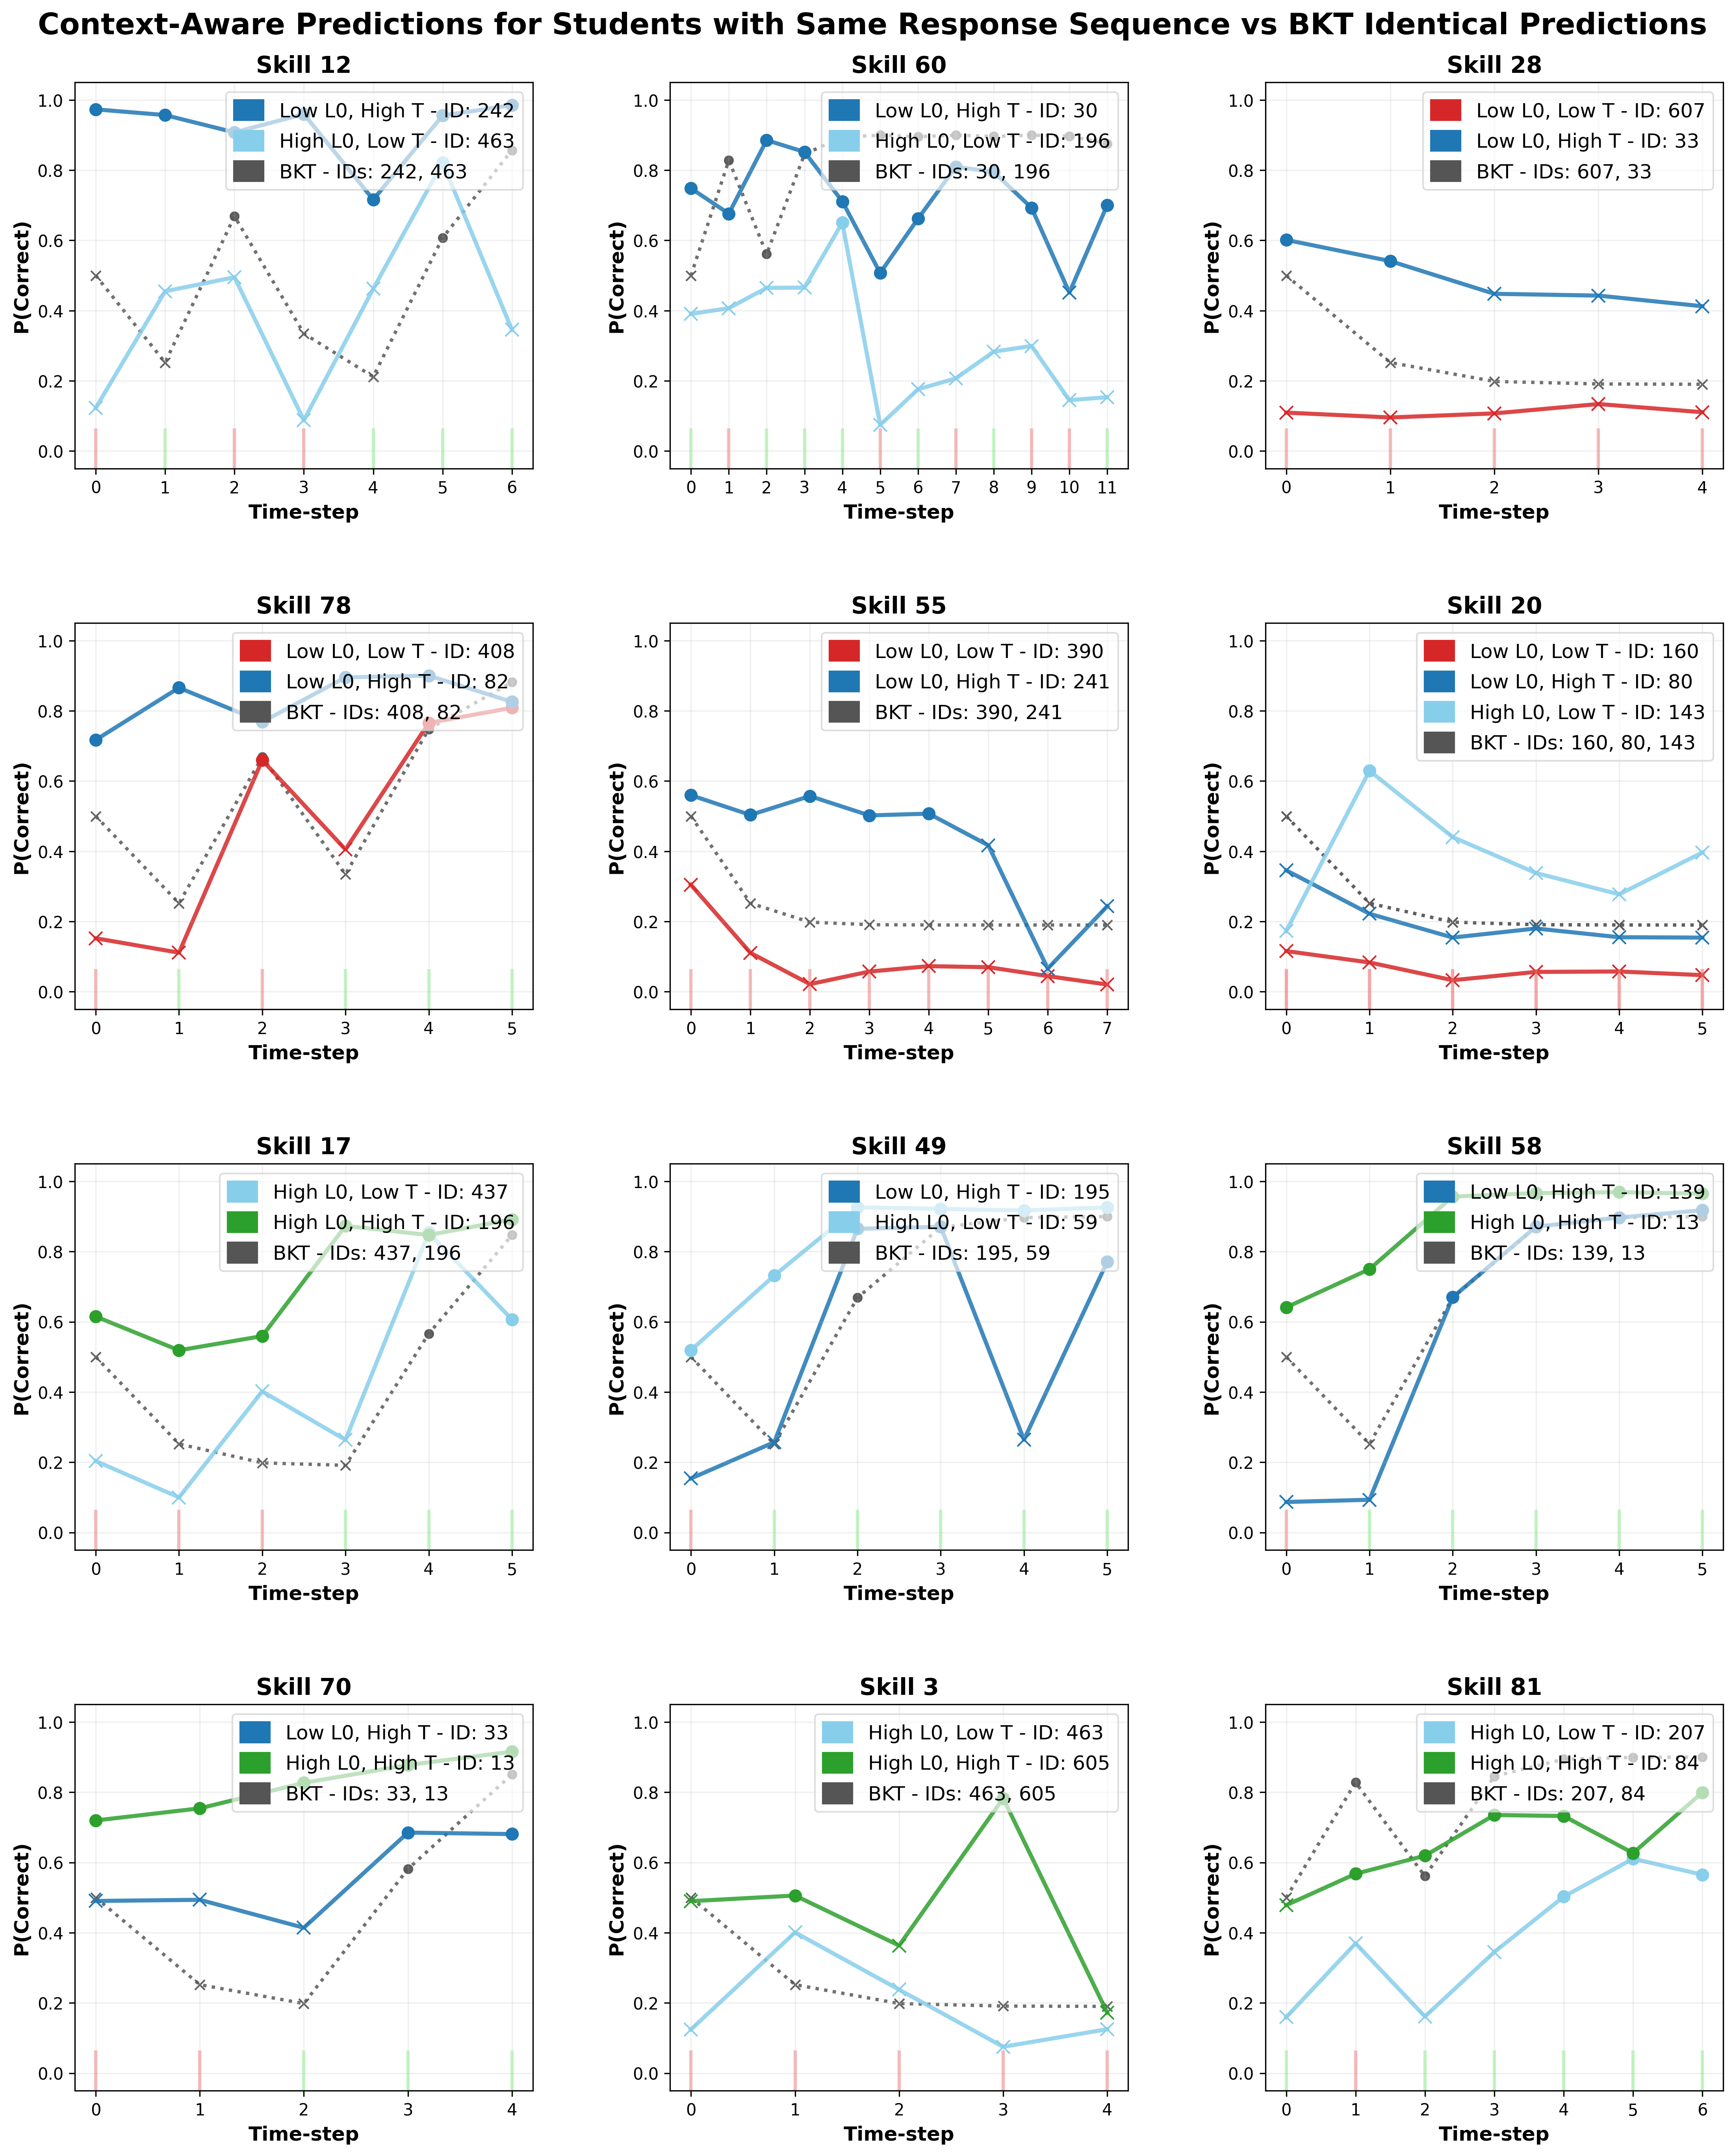
\includegraphics[width=\textwidth]{h3_skill_quadrant_comparison_mosaic_893468.png}
\caption{\textbf{Context-aware prediction mosaic.} Each panel shows students with identical response sequences (green/red bars for correct/incorrect responses) but different learning situations. BKT predictions (dotted grey) overlap due to Markovian constraints; gTransformer predictions (solid coloured) diverge based on historical parameters ($p_{\text{L}_0}$, $p_{\text{T}}$). Circles indicate predicted correct responses; crosses indicate predicted failures.}
\label{fig_mosaic}
\end{figure}

This divergence has direct implications for the tutorial model. Each student interaction event can be routed to a different instructional pathway based on the learning situation assigned by gTransformer. A student whose trajectory places them in situation (1) triggers a scaffolding strategy; a student in situation (4) is routed towards accelerated content progression. Crucially, this routing is not static: as new interactions arrive, gTransformer updates its parameter estimates from the full longitudinal context, allowing the tutorial model to dynamically reassign students across situations as their learning trajectory evolves. This event-driven, context-aware routing is precisely what population-level models such as standard BKT cannot support---two students with an identical recent response pattern may receive different instructional interventions if their prior histories place them in different learning situations.

%
\section{Discussion}

\subsection{Theory-Grounded Instructional Decisions}

The results demonstrate that gTransformer addresses the accuracy--interpretability trade-off in KT by providing pedagogically grounded parameters at a minimal performance cost. This is directly relevant to the ECTEL 2026 theme of Mindful TEL: the model embodies the principle that learning technologies should be shaped with intention, ensuring that the cognitive engine of an ITS is anchored in established educational theory rather than opaque data-driven heuristics.

By operationalising BKT parameters ($P_{\text{L}_0}$, $P_{\text{T}}$) derived from deep learning context, gTransformer provides educators with the diagnostic handles through which an ITS can perform mindful instruction. Rather than acting as a black box that issues recommendations without justification, the system grounds its decisions in constructs that practitioners recognise and can validate. This aligns with broader EU imperatives for explainable, accountable AI in education~\cite{Holmes2022504}, and responds directly to the concerns raised by the Artificial Intelligence Act's designation of educational AI as high-risk.

\subsection{Beyond Static Labelling: Context-Aware Adaptation}

A central contribution of this work is the shift from population-level labelling to situation-based diagnosis. The results presented in Section~\ref{sec_personalisation} demonstrate that gTransformer's context-aware predictions provide a higher-resolution understanding of the learning journey than population-level models. By encoding each student's longitudinal history into personalisable parameters, the model acknowledges that students are dynamic learners whose instructional needs evolve continuously.

This enables educators to identify, for instance, students with high prior knowledge but low learn rate---suggesting disengagement or instructional mismatch---and adapt the pacing accordingly before significant learning gaps emerge. Conversely, students with high prior knowledge and high learn rate can be identified for accelerated progression to prevent unnecessary remediation. This intentional design addresses essential concerns about accountability and pedagogical integrity in automated instruction.

\subsection{Pedagogical Integrity and Human Agency}

The triple-validation methodology (RQ2) establishes that the model's internal representations genuinely internalise pedagogical theory rather than merely correlating with it. Structural alignment confirms BKT constructs as primary organising principles; semantic alignment confirms that grounded parameters retain their pedagogical semantics; and functional alignment quantifies the confidence with which educators can trust interpretable predictions. Together, these results support the claim that gTransformer is not merely a high-performance prediction system, but a theory-grounded diagnostic tool that can serve as the cognitive foundation of responsible, human-centred ITS.

%
\section{Conclusions}

This work demonstrates how gTransformer~\cite{labra2026theory}, a Grounded Transformer that bridges deep learning performance and pedagogical interpretability through \textit{representational grounding}, can serve as the cognitive foundation of a theory-grounded ITS. We evaluated its capacity to instantiate the three core ITS components. As a user model, interpretable gTransformer predictions consistently surpass classical BKT with an average gain of 19.9\% AUC, at a low interpretability cost of 3.9\% relative to black-box architectures. As a domain model, gTransformer internalises BKT constructs as its primary organising principle in latent representations, confirmed by structural, semantic, and functional alignment. As a tutorial model foundation, gTransformer enables context-aware, situation-based instruction by capturing longitudinal learning patterns that Markovian models cannot represent.

As a foundation for TEL, gTransformer demonstrates that pedagogically justifiable student modeling is achievable without sacrificing the predictive power needed for effective adaptive instruction. The \textit{representational grounding} methodology is domain-independent and may be extended to other theoretical frameworks beyond BKT or to other scientific fields where established theoretical models coexist with high-volume empirical data. Future research will investigate the integration of guess and slip parameters for finer-grained personalisation and the generalisation of gTransformer to alternative educational theories.

%
\begin{credits}
\subsubsection{\ackname}
This research received no external funding.

\subsubsection{\discintname}
The authors have no competing interests to declare that are relevant to the content of this article.
\end{credits}

%
\bibliographystyle{splncs04}
\bibliography{biblio}

\end{document}
